\documentclass{journal}
\usepackage{graphicx}
\usepackage{epstopdf}
\usepackage{overpic}
\usepackage{color}
\usepackage{amsmath}
\usepackage{amsfonts}
\usepackage{amsthm}
\usepackage{svg}


\theoremstyle{definition}
\newtheorem{definition}{Definition}
\newtheorem{theorem}{Theorem}
\newtheorem{lemma}{Lemma}
\newtheorem{corollary}{Corollary}
\newtheorem*{remark}{Remark}

\begin{document}
\title{A Computational Model of Binge Drinking in Social Networks}
\maketitle

\section*{Background}

Individual propensity for alcoholism has been modeled using the bistable rate function
\[
\frac{dv}{dt} = v(1-v)a
\]
where $a$ is determined by an individual's resilience and surrounding peer pressure in the social network  \cite{Braun2010, Braun2006}. In this model, an individual's propensity to drink evolves towards alcoholism ($v=1$) or sobriety ($v=0$) depending on the sign of $a$. This differential equation is similar to the equations used in SIR models in that it describes the evolution of a population from initial conditions to a steady state. Unlike the SIR model, individuals remain in a state of permanent alcoholism or sobriety at the end of the modeling process. The work in \cite{Braun2006} also investigates the impacts of treating a percentage of of the population for alcoholism and found that if roughly 7\% of the population is treated, the whole population returns to sobriety.

Other, more complicated models to study this phenomenon are also proposed and some are studied with perturbation theory in \cite{Braun2010}. Our work differs from the results presented above in that our work models each drink taken and the work above studies alcoholism in aggregate. Our work is a finer grained model of similar phenomenon. Additionally, \cite{Braun2010} focuses on analytic results but we focus on aligning our model output with collected data.

A 2020 review surveyed the use of complex system techniques for modeling alcohol use \cite{Mcgill2020}. These techniques vary from conceptual models to computational models. The computational models fall mainly into two categories, systems level models and agent based models. The systems level models divide the population into cohorts and use data to provide estimate rate parameters to describe the rate at which individuals move between cohorts. For example, a model might contain the rate at which moderate drinkers become heavy drinkers and this would be estimated from data. These models behave in a manner similar to SIR models for infectious disease. Usually these models are somewhat tractable analytically and lend themselves to fixed point and stability analysis.

The second main approach, agent based models, focus on the behavior of individuals. The models specify rule by which autonomous individuals may interact with the environment. These models are usually intractable analytically and are therefore studied via repeated simulations across different parameters.

WHO defines this binge drinking based on the consumption of 5 to 6 glasses of alcohol per occasion.

\section*{Model Description}
\begin{figure}[h] \label{fig:nonuniform_person}
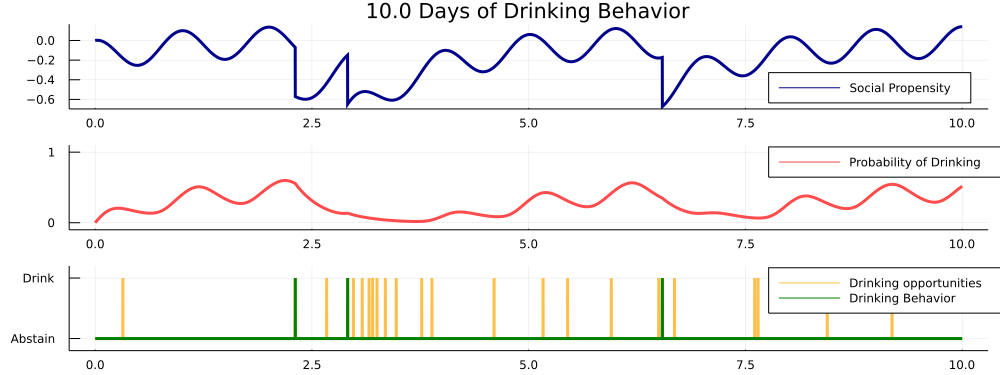
\includegraphics[width=\textwidth]{nonuniform_person.png}
\caption{A realization of model state variables for mood function $m(t) = \sin(2\pi t)$ and $E = \{ t_0, t_1, t_2, ...\}$ where $t_{i+1} - t_i$ is drawn from an exponential distribution with rate parameter equal to 1.}
\end{figure}
Our model of a social drinker is governed by the following equations. 

\begin{align}
\frac{ds}{dt} = s_{\text{slope}}s + m(t)  \\
\frac{dp}{dt}  = \gamma[-p + \sigma\,(a s) + b] \\
s(t_i) \leftarrow s(t_i) - s_{drink} \quad \text{if } t_i \in e 
\end{align}

where $s$ represents an individuals propensity to be social, $p$ represents probability of drinking (if alcohol is encountered), $m(t)$ is given and represents mood, and $e$ is a given set of encounter times. Together these equations model an individual's drinking behavior. This model can be classified as a switched dynamical system, but not in the true sense, because there is only a single function governing the continuous dynamics. In the following sections, we provide some intuition for what each of the model variables and parameters mean.

\subsection*{Propensity To Drink Socially ($s$)}

This variable represents a person's desire to drink socially. It increases when they are in a good mood and decreases when they are in a bad mood. Upon drinking, $s$ immidiately makes a discontinuous jump down. This models an individuals ability to regulate their own social drinking. The size of this instantanious decrease $s_{drink}$ is a parameter that can be tuned to match different kinds of behavior. A large $s_{drink}$ might model an individual who doesn't like to drink a lot in quick succession. in the period following drinking, if the individual does not drink again, their desire to drink socially will return to normal levels. The speed at which it returns to normal levels is governed by $s_{slope}$, which is also a parameter that can be tuned.

\subsection*{Probability of Drinking ($p$)}

The variable $p$ represents a person's probability of drinking at a given time. It's evolution depends on the evolution of $s$. The trajectory of $p$ usually looks like a transformed version of $s$ that stays in the interval (0,1). The responsiveness of $p$ to $s$ is governed by the parameter $\gamma$. This parameter controls the delay, or how quickly $p$ changes in response to changes in $s$. For large $\gamma$, every change in $s$ will be reflected in the trajectory of $p$. For small $\gamma$, small scale oscillations in $s$ will not affect $p$, and $p$ will tend to illustrate the longer term trends present in the evolution of $s$. The parameter $a$ controls the impact of $s$ on $p$ and is usually set to $a=10$. The parameter $b$ controls the probability of drinking when an individual is in a neutral mood.

\subsection*{Drinking Opportunities ($e$)}

In this model, the modeler supplies two pieces a priori, a function describing an individual's mood at a given time, $m(t)$, and a set of times that an individual will encounter alcohol, $e$. Before an encounter time is reached, $s$ and $p$ evolve according to differential equation outlined above and respond to the individual's mood. When an encounter time $t_i \in e$ is reached, a draw is taken from a bernoulli random variable with probability of success equal to $p(t_i)$. (This is essentially a coin that lands on heads with probability $p(t_i)$.)

If the random draw is equal to one, the model records that a drink was taken at time $t_i$, and decreases the current value of $s$ by $s_{drink}$.  If the random draw is zero, nothing changes.
Afterwards, the model continues to evolve according to the differential equation until the next drinking opportunity.

\subsection*{Coupling Multiple Individuals}

To couple together the drinking of multiple people, we use a simple rule. Each time I drink, my neighbors in the social network are given an opportunity to drink at the next time-step. This rests on the idea that if my friends go out and drink, I am likely to get invited to go with them. We implement this as follows. If person $i$ drinks at time $t$, and has neiggbors $j_1, ..., j_m$, then we update the set of event $e_{j_k}$ times belonging to each neighbor to include the time $t + \delta t$ where $\delta t$ is the model time-step.

\section*{Model Statistics}

\subsection*{Drinking Stats}
\begin{figure}[h] \label{fig:uniformdrinker}
	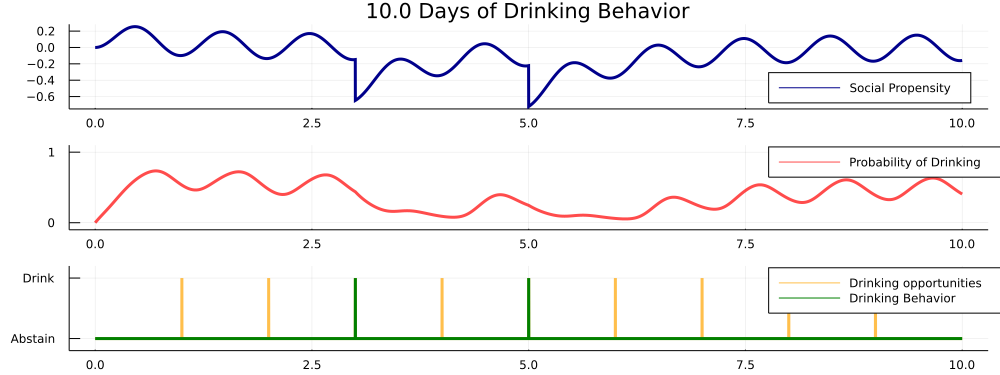
\includegraphics[width=\textwidth]{uniform_person.png}
	\caption{One realization of model state variables for a drinker with mood function $m(t) = sin(2\pi t) $ and event times $E = \{1, 2, ... 10\}$. In this realization, the individual takes drinks at $t=3$ and $t=5$. The red curve here is one of 1000 realizations plotted in Figure \ref{fig:expectedp}.}
\end{figure}

Assume that $e$ and $m$ are fixed. Let $\mathbf{d}(t)$ represent a stochastic sequence of drinks. Because of the model construction, we can write 
\begin{align*}
\mathbf{d}(t) = \sum_i^{|e|} \delta (t - t_i)\mathbf{B}(\mathbf{p}(t_i))
\end{align*}
Where $\delta$ is the Dirac delta function, $\mathbf{B}(p)$ is a Bernoulli random variable with parameter $p$, and $\mathbf{p}(t_i)$ is the drinking probability stochastic process generated by the model.

Then, the random variable for number of drinks is defined as 
\[
\mathbf{D} = \int_0^T \mathbf{d}(t)dt = \sum_{i=1}^{|e|} \mathbf{B}(\mathbf{p}(t_i))
\]
and the expectation of $\mathbf{D}$ is
\begin{equation} \label{equ:expectdrink}
\mathbb{E}[\mathbf{D}] = \sum_{i=1}^{|e|}\mathbb{E}[\mathbf{B}(\mathbf{p}(t_i))] = \sum_{i=1}^{|e|} \mathbb{E}[\mathbb{E}[\mathbf{B} \, | \, \mathbf{p}(t_i))]] = \sum_{i=1}^{|e|} \mathbb{E}[\mathbf{p(t_i)}] = \sum_{i=1}^{|e|} \mathbb{E}[\mathbf{p(t_i)}]
\end{equation}

Thus, the expected number of drinks depends completely on the expected probability of drinking function $\mathbb{E}[\mathbf{p(t)}]$. The current model does not allow an analytic solution for $p(t)$ given a sequence of drink decisions, but if it was modified so that an analytic solution existed we might be able to solve for $\mathbb{E}[\mathbf{p(t_i)}]$ pseudo-explicitly. Otherwise the best we can do is simulation and averaging.

To get a clearer picture of the stochasiticity of the solution, we use a simple oscillating mood function $m(t) = sin(2\pi t)$ and regular drinking opportunity times $E = \{1, 2, 3, ...\}$. A single realization using these opportunity times and mood function is plotted in Figure \ref{fig:uniformdrinker}.

\begin{figure}[h] \label{fig:expectedp}
	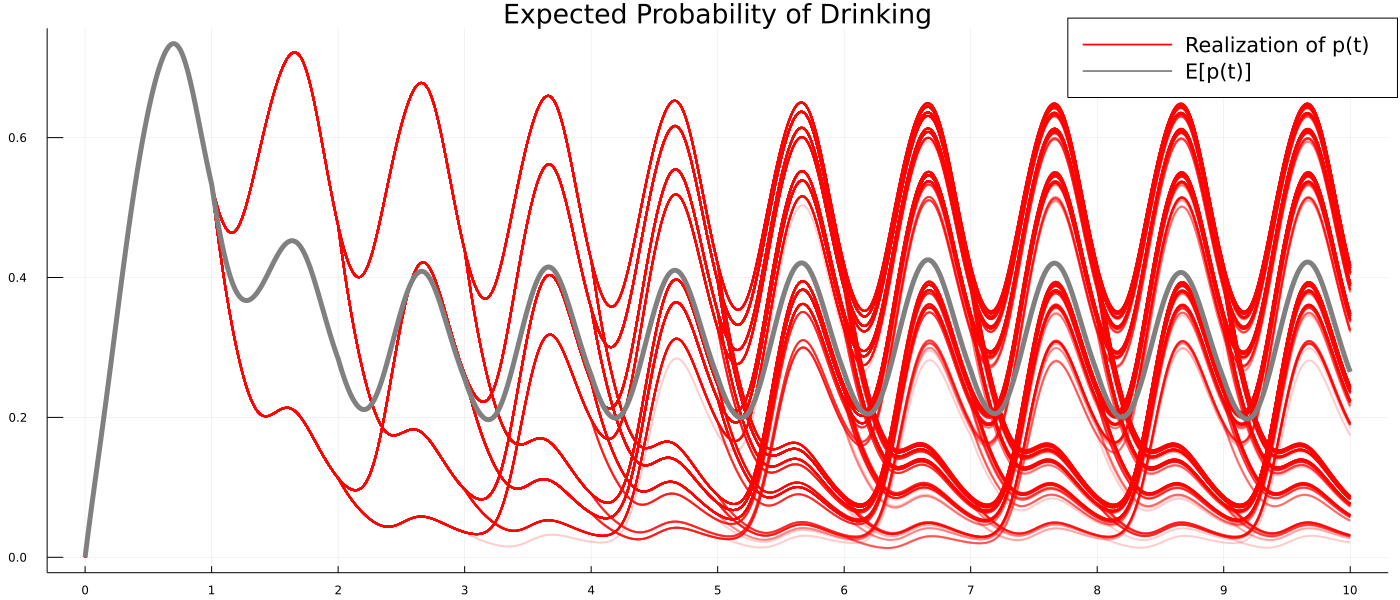
\includegraphics[width=\textwidth]{expected_p.png}
	\caption{This plot shows 1000 realizations of $\mathbf{p}(t)$ in red, as well as the mean value of all realizations in gray. }
\end{figure}

Figure \ref{fig:expectedp} shows 1000 realizations of $\mathbf{p}(t)$ simulated with $m(t)$ and $e$ defined above. At each drinking opportunity, a portion of the realizations drink and a portion do not. This creates a branching structure in the realizations. Before the first drinking opportunity at $t=1$, all realizations follow the same path. Afterwards, they split into two paths, the realizations that drink at $t=1$ and those that do not. At time $t=2$ there are 4 unique paths and etc.. What is interesting, is that the realizations do not spread out uniformly, rather, they stay clustered together in common paths. This may be due to the structure of the differential equation, for example, this clustering could be a property of the exponential decay in $s(t)$ and $p(t)$.

\section{A Simpler Model}

We simplify our problem to a single variable, probability of drinking $p$, and accept a mood function $m(t)$ and a set of drinking opportunities $e$ .

\[ 
\frac{dp}{dt} = a\big(-p(t) + m(t)\big) 
\]

The if $p(t_0) = p_0$, solution to this equation is 

\begin{equation}
\label{equ:simplemodel}
p(x) = e^{-at} \int_{t_0}^t -ae^{as}m(s)ds + p_0 e^{-a(t-t_0)}
\end{equation}

We add in a probabilistic drinking just like before. Drinking reduces the probability of drinking.

\begin{equation}
\label{equ:simplemodelupdate}
 p(t_i) \leftarrow p(t_i) - b\text{ with probability } p(t_i) \text{ if } t_i \in e
\end{equation}

Where b is a fixed parameter representing the amount that probability of drinking decreases in response to a drinking event. To keep $0 \leq p \leq 1$ we require $0 \leq m(t) \leq 1$ for all $t$ and in the case that $p(t_i) - b < 0$, we set $p(t_i) \leftarrow 0$ to avoid negative probabilities. 

Using $ a=1.2, b=.2$ and $m(t) = .5$ or $m(t) = \frac{1}{2}\big(\sin(2\sqrt{2}\pi (t - 1/4)) + 1\big)$ with drinking opportunities at $E = \{1, 2, 3, ...\}$ produces Figure \ref{fig:simple_expected_p}.

\begin{figure}[h] \label{fig:simple_expected_p}
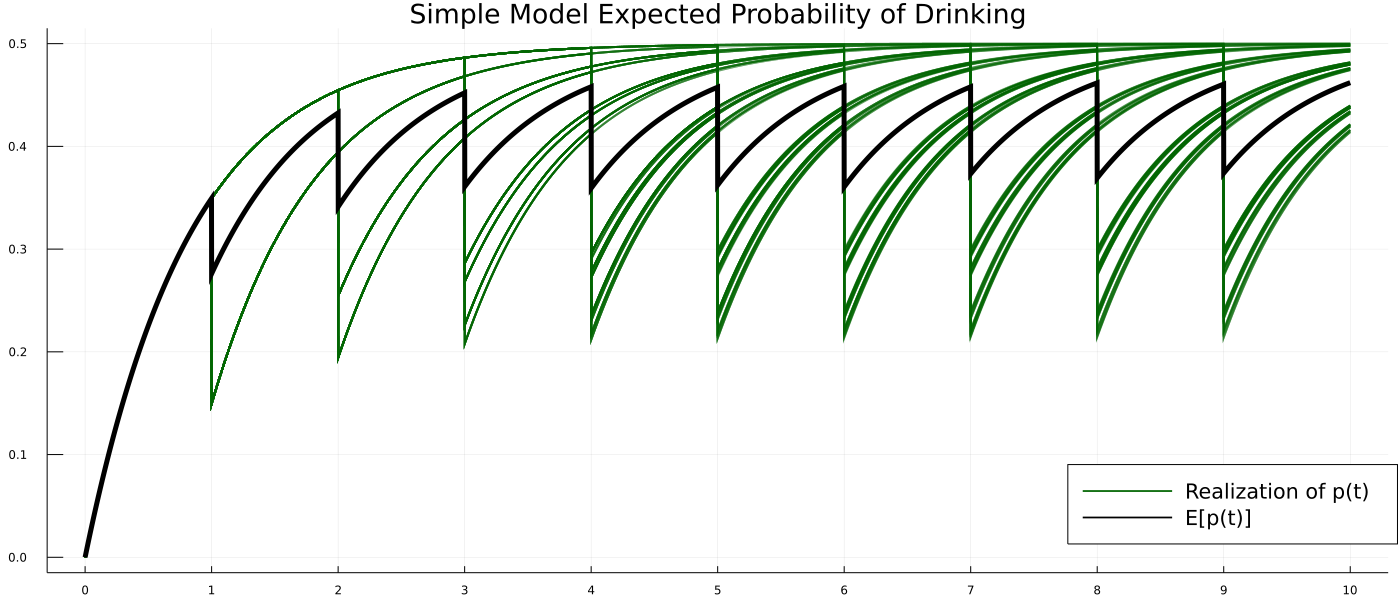
\includegraphics[width=0.5\textwidth]{simple_expected_p.png}
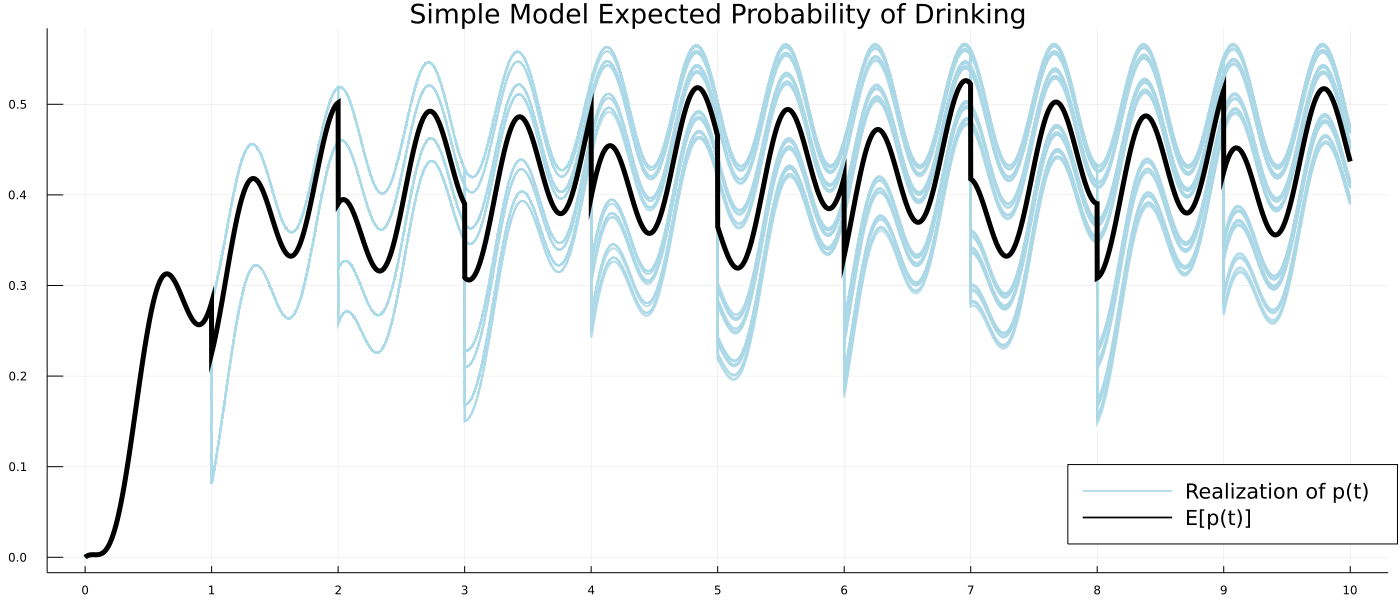
\includegraphics[width=0.5\textwidth]{simple_expected_p_sin.png}
\caption{Results of simulating a single variable stochastic model (see Equations \ref{equ:simplemodel} and \ref{equ:simplemodelupdate}) with probabilistic updates. A constant mood function was used for the plot on the left and a $m(t) = \frac{1}{2}\big(\sin(2\sqrt{2}\pi (t - 1/4)) + 1\big)$ was used for the plot on the right. The results of 300 different simulations are plotted in green and blue and the mean of all simulations, $\mathbb{E}[\mathbf{p(t)}]$, is plotted in black. Note that the top colored curve represents the evolution of the system without any discontinuous jumps down, i.e. the system without any stochasticity. It is interesting to note that the average over all the simulations, $\mathbb{E}[\mathbf{p(t)}]$ (black) appears lower than this by a fixed amount and appears to have some regularity. We derive a closed form for this black curve later.}
\end{figure}

\subsection{A Closed Form for $\mathbb{E}[\mathbf{p(t)}]$}

As shown in equation \ref{equ:expectdrink}, the expected number of drinks is solely dependent on $\mathbb{E}[\mathbf{p(t)}]$. ($\mathbb{E}[\mathbf{p(t)}]$ is the expectation of the stochastic process $\mathbf{p}(t)$ that is generated by the differential equation with stochastic updates.) Then, if we want to know how many drinks the model will produce for a given set of parameters, all we need is $\mathbb{E}[\mathbf{p(t)}]$. This can be computed approximately by running many simulations and averaging, but it is much less costly to obtain a closed form.

\begin{definition}[Event Stochastic Linear System]\label{def:esls}
An event stochastic linear system is the combination of a linear first order differential equation, a linear probability density function $p(x) = \alpha x + \beta$,  a set of event times $E = \{t_1, t_2, ..., t_N\}$ and an update function $g$ of the form $g(x) = x + c$ where $c$ is a constant. We can write this system in the form:
\begin{equation}\label{equ:def_cont_dyn}
\frac{dx}{dt} = a\big( -x(t) + m(t) \big), \quad x(t_0) = x_0
\end{equation}
\begin{equation}\label{equ:def_prob_dyn}
x(t_i) \leftarrow g(x(t_i)) \text{ with probability } p(x(t_i))
\end{equation}
where Equation \ref{equ:def_cont_dyn} defines the continuous dynamics and \ref{equ:def_prob_dyn} defines discrete stochastic dynamics. We additionally let the state variable $x(t_i)$ to be equal to the updated value (if an update occurs) so that the solution is left continuous and not right continuous.
\end{definition}

The solution to a Event stochastic linear system is a discrete random variable $\mathbf{x}(t)$. There are $2^N$ distinct curves that could appear in a simulation. This is because at each event, the system make a decision between 2 different paths. With no events, there is a single distinct path. If there is one event, there are two possible distinct paths, for two events, the paths branch a second time producing four unique paths and etc.

Each of these paths occurs with a different probability, depending on the state of the system before the event and the probability density function.

We note that $p(x)=\alpha x + \beta$ must remain within $[0, 1]$ for all $x$ generated by the system, otherwise the event stochastic ode is not well defined. This means that $\mathbf{x}(t) \in [\frac{-\beta}{
alpha}, \frac{1-\beta}{\alpha}]$ for all $t$.  It is not always clear that this will be the case. If $a$ is positive and $m(t)$ is bounded, the continuous dynamics are bounded and stable. As long as the constant $c$ in the update function $g(x) = x+c$ is small relative to the time between events, the solutions should remain bounded. In this case, there should be appropriate $\alpha$ and $\beta$ to map $x$ values to probabilities. Whether such $\alpha$ and $\beta$ exist when the continuous dynamics are unstable, or when $c$ is large relative to the time between events remains to be seen.

\begin{definition}[Piece-Wise Expectation]\label{def:piece}
Given an event stochastic linear system with event times $E = \{t_1, t_1, ..., t_N\}$, we define the piece-wise expectation $\mu_i(t)$ to be $\mu_i(t) = \mathbb{E}[\mathbf{x(t)}]$ on the interval $[t_{i-1}, t_i)$ and $\mu_i(t_i)$ to be the expected value of the solutions \textit{prior to the stochastic update}. Therefore $\mu_{i+1}(t_i) = \mathbb{E}[\mathbf{x(t_i)}] \neq \mu_i(t_i)$ in general.
\end{definition}

Before proceeding, we note that the solution to the system in Equation \ref{equ:def_cont_dyn} without stochasticity is
\begin{equation*} 
x(t) = \int_{t_0}^t -ae^{a(s-t)}m(s)ds + x_0 e^{-a(t-t_0)}
\end{equation*}
when the initial data is $x(t_0) = x_0$.

To simplify notation later we define $I_i(t) = \int_{t_{i-1}}^t -ae^{a(s-t)}m(s)ds$ so that
\begin{equation} \label{equ:cont_sol}
x(t) = I_1(t) + x_0 e^{-a(t-t_0)}
\end{equation}

Because we want to derive the $\mathbb{E}[\mathbf{x(t)}]$ for all $t$, we need a way to relate the behavior of $\mu_i$ to the behavior of $\mu_{i+1}$.

\begin{lemma} \label{thm:update_relate}
\textit{Given an event stochastic linear system (see Definition \ref{def:esls}). with event times $E = \{t_1, t_2, ... t_N\}$, probability function $p(x)$, and piece-wise expectation $\{\mu_i(t)\}_{i=1}^N$, it must be the case that:
\begin{equation}\label{equ:update_relate}
\mu_{i+1}(t_i) = cp\big(\mu_i(t_i)\big) + \mu_i(t_i)
\end{equation}
}
\end{lemma}

\begin{proof}
Assume that $\{x_k(t)\}_{k=1}^{M}$ are $M$ sampled solutions to the given event stochastic  linear system that are valid on the interval $[t_0, t_i)$. However, we also assume that each $x_k(t_i)$ has not yet received a stochastic update. Then,
\[
\mu_i(t) = \lim_{M\rightarrow \infty} \frac{1}{M} \sum_{k=1}^M  x_k(t)
\] on the entire interval $[t_i-1, t_i].$
We know that $\mu_{i+1}(t_i)$ is equal to the average of the sampled solutions after they receive their stochastic update. For a particular solution $x_k(t)$, the expected value after the stochastic updated is 
\[
p(x_k(t))\big(x_k(t) + c \big) + \big[1 - p(x_k(t))\big]x_k(t).
\] 
This is because the update occurs with probability $p(x_k(t))$ and does not occur with probability $1 - p(x_k(t))$. Thus, 
\begin{flalign*}
\mu_{i+1}(t_i)  &= \lim_{M\rightarrow \infty} \frac{1}{M} \sum_{k=1}^M p(x_k(t_i))\big( x_k(t_i) + c \big) + \big[1 - p(x_k(t_i))\big]x_k(t_i) \\
&= \lim_{M\rightarrow \infty} \frac{1}{M} \sum_{k=1}^M p(x_k(t_i)) x_k(t_i) + c p(x_k(t_i)) + x_k(t_i) - p(x_k(t_i))x_k(t_i)  \\
&=  c p \Big(\lim_{M\rightarrow \infty} \frac{1}{M} \sum_{k=1}^M x_k(t_i) \Big) + \lim_{M\rightarrow \infty} \frac{1}{M} \sum_{k=1}^M x_k(t_i) \\
 &= cp(\mu_i(t_i)) + \mu_i(t_i)
\end{flalign*}
This concludes the proof.
\end{proof}
\begin{remark}
Note that Lemma \ref{thm:update_relate} shows that at an event time, $t_i$, the expectation of the updated paths is equal to the expected valued of an update applied to the mean final values. This proof technique only works for linear $p(x)$ and $g(x)$ of the form $g(x) = x + c$. It is possible that the statement is not true for any other kinds of density and update functions.
\end{remark}

Before writing an explicit formula for $\mathbb{E}[\mathbf{x(t)}]$, we need another result.

\begin{corollary} \label{thm:piece_relate}
For an event stochastic linear system (see Definition \ref{def:esls}) with event times $E = \{t_1, t_2, ... t_N\}$, probability density function $p(x) = \alpha x + \beta$, initial data $x(t_0) = x_0$, and piece-wise expectation $\{\mu_i(t)\}_{i=1}^N$, and $I_i(t) = \int_{t_{i-1}}^t -ae^{a(s-t)}m(s)ds$, we can write $\mu_{i+1}(t)$ in terms of $\mu_{i}(t_i)$. Explicitly,
\[
\mu_{i+1}(t) =I_{i+1}(t) + c\beta e^{-a(t-t_i)} + (c\alpha + 1)\mu_i(t_i) e^{-a(t-t_i)}
\]
and
\[
\mu_1(t) = I_1(t) + x_0e^{-a(t-t_0)}
\]
\end{corollary}

\begin{proof}
Assume that $\{y_k(t)\}_{k=1}^{M}$ are $M$ sampled solutions to the given event stochastic  linear system that are valid on the interval $[t_0, t_i]$, that is, assume that each $y_k(t_i)$ has received a stochastic update.

Then, the continuation of a particular $y_k(t)$ in to the interval $[t_i, t_{i+1})$ is  defined as the solution to Equation \ref{equ:def_cont_dyn}, defined in Equation \ref{equ:cont_sol}. That is
\[
y_k(t) = I_i(t) + y_k(t_i) e^{-a(t-t_i)} \quad t \in [t_i, t_{i+1}).
\]
Then,
\begin{flalign*}
\mu_{i+1}(t) &= \lim_{M\rightarrow \infty} \frac{1}{M} \sum_{k=1}^M y_k(t_i) \\
&= \lim_{M\rightarrow \infty} \frac{1}{M} \sum_{k=1}^M I_i(t) + y_k(t_i) e^{-a(t-t_i)} \\
&= I_i(t) + e^{-a(t-t_i)} \lim_{M\rightarrow \infty} \frac{1}{M} \sum_{k=1}^M y_k(t_i) \\
&= I_i(t) + \mu_{i+1}(t_i)e^{-a(t-t_i)} \\
\end{flalign*}
Then, applying Corollary \ref{thm:piece_relate} produces
\begin{flalign*}
\mu_{i+1}(t) &= I_i(t) + \big( cp(\mu_i(t_i)) + \mu_i(t_i) \big) e^{-a(t-t_i)} \\
&= I_i(t) + \big( c\alpha\mu_i(t_i) + c\beta + \mu_i(t_i) \big) e^{-a(t-t_i)} \\
&= I_i(t) + c\beta e^{-a(t-t_i)} + (c\alpha + 1)\mu_i(t_i) e^{-a(t-t_i)} \\
\end{flalign*}
as required.

Lastly, we note that on the interval $[t_0, t_1)$, no event has occurred, so there is no stochasticity. Thus every solution is the same on this interval and depends only on the initial data:
\[
\mathbf{x}(t) = I_1(t) + x_0e^{-a(t-t0)}
\]
for $t \in [t_0, t_1)$. Thus, in this interval
\[
\mathbb{E}[\mathbf{x}(t)] = I_1(t) + x_0e^{-a(t-t0)}
\]
implying that 
\[
\mu_1(t) = I_1(t) + x_0e^{-a(t-t0)}
\].
Thus we have found a recurrence relation for the piece-wise expectation, $\mu_i(t)$.
\end{proof}

\begin{theorem}[Expectation of an event stochastic linear system] \label{thm:expectation}
Let $\mathbf{x}(t)$ be a random variable representing the solution to an event stochastic linear system, with probability density function $p(x) = \alpha x + \beta$, event times $E = \{t_1, t_2, ..., t_N\}$ and update function $g(x) = x + c$, with continuous dynamics governed by
\begin{equation*}
\frac{dx}{dt} = a\big( -x(t) + m(t) \big), \quad x(t_0) = x_0
\end{equation*}
and probabilistic updates governed by
\begin{equation*}
x(t_i) \leftarrow g(x(t_i)) \text{ with probability } p(x(t_i))
\end{equation*}.

Then, for $t \in [t_{n-1}, t_n)$, the expected value of the solution is 
\begin{equation} \label{equ:piece_sol}
 \mathbb{E}[\mathbf{x}(t)] = I_n(t) + w_ne^{-at}
\end{equation}
where 
\begin{equation} \label{equ:exp_weights}
w_n = (c\alpha + 1)^{n-1} x_0 e^{at_0} + \sum_{k=1}^{n-1} (c\alpha +1)^{n-k}\big(\frac{c\beta}{c\alpha +1} + I_{k}(t_{k})\big)e^{at_{k}} 
\end{equation}
and
\[
I_i(t) = \int_{t_{i-1}}^t -ae^{a(s-t)}m(s)ds \quad i \in \{1, ..., N \}.
\]
\end{theorem}

\begin{proof}
By definition of $\mu_n(t)$,  $\mathbb{E}[\mathbf{x}(t)]  = \mu_n(t)$. Thus it suffices to show that 
\[
\mu_n(t) =I_n(t) + w_ne^{-at}
\]
as defined above. By Corollary \ref{thm:piece_relate} we have
\[
\mu_n(t) = I_{n}(t) + c\beta e^{-a(t-t_{n-1})} + (c\alpha + 1)\mu_{n-1}(t_{n-1}) e^{-a(t-t_{n-1})}.
\]
Applying Corollary \ref{thm:piece_relate} again to $\mu_{n-1}(t_{n-1})$ gives
\begin{multline*}
\mu_n(t) = I_{n}(t) +  c\beta e^{-a(t-t_{n-1})} \\
+ (c\alpha + 1)\Big( I_{n-1}(t_{n-1}) + c\beta e^{-a(t_{n-1}-t_{n-2})}  \\
+ (c\alpha + 1)\mu_{n-2}(t_{n-2}) e^{-a(t_{n-1}-t_{n-2})}\Big)e^{-a(t-t_{n-1})} 
\end{multline*}
which produces
\begin{multline*}
\mu_n(t) = I_{n}(t) +  \Big( c\beta + (c\alpha +1) I_{n-1}(t_{n-1}) \Big) e^{-a(t-t_{n-1})} \\
+ \Big( (c\alpha +1) c\beta  + (c\alpha +1 )^2 \mu_{n-2}(t_{n-2})\Big) e^{-a(t - t_{n-2})}.
\end{multline*}
Applying Corollary \ref{thm:piece_relate} $n-1$ more times,  we derive
\begin{multline*}
\mu_n(t) = I_{n}(t) +  \Big( c\beta + (c\alpha +1) I_{n-1}(t_{n-1}) \Big) e^{-a(t-t_{n-1})} \\
+ \Big( (c\alpha +1) c\beta  + (c\alpha +1 )^2 I_{n-2}(t_{n-2})\Big) e^{-a(t - t_{n-2})} \\
+ \cdots \\
+ \Big( (c\alpha +1)^{n-3} c\beta  + (c\alpha +1 )^{n-2} I_{2}(t_{2})\Big) e^{-a(t - t_{2})} \\
+ \Big( (c\alpha +1)^{n-2} c\beta  + (c\alpha +1 )^{n-1} \mu_1(t_1)\Big) e^{-a(t - t_{0})}.
\end{multline*}
Recalling that $\mu_1(t_1) = I_1(t_1) + x_0e^{t_1 - t_0}$ produces:
\[
\mu_n(t) = I_n(t) + \sum_{k=1}^{n-1} (c\alpha +1)^k\Big(\frac{c\beta}{c\alpha +1} + I_{n-k}(t_{n-k})\Big)e^{-a(t-t_{n-k})} + (c\alpha + 1)^{n-1} x_0 e^{-a(t-t_0)}
\]
Reindexing ($k = n-k$) gives the desired result.
\begin{flalign*}
\mu_n(t) &= I_n(t) 
+ \sum_{k=1}^{n-1} (c\alpha +1)^{n-k}\Big(\frac{c\beta}{c\alpha +1} + I_{k}(t_{k})\Big)e^{-a(t-t_{k})} 
+ (c\alpha + 1)^{n-1} x_0 e^{-a(t-t_0)} \\
&= I_n(t) + e^{-at}\Big( \sum_{k=1}^{n-1} (c\alpha +1)^{n-k}\big(\frac{c\beta}{c\alpha +1} + I_{k}(t_{k})\big)e^{at_{k}} 
+ (c\alpha + 1)^{n-1} x_0 e^{at_0} \Big)
\end{flalign*}
 This concludes the proof of a closed from for the expectation of $\mathbf{x}(t)$.
\end{proof}

\subsection{Numerical Verification of the Analytic formula for $\mathbb{E}[\mathbf{x}(t)]$}

\begin{figure}[h]
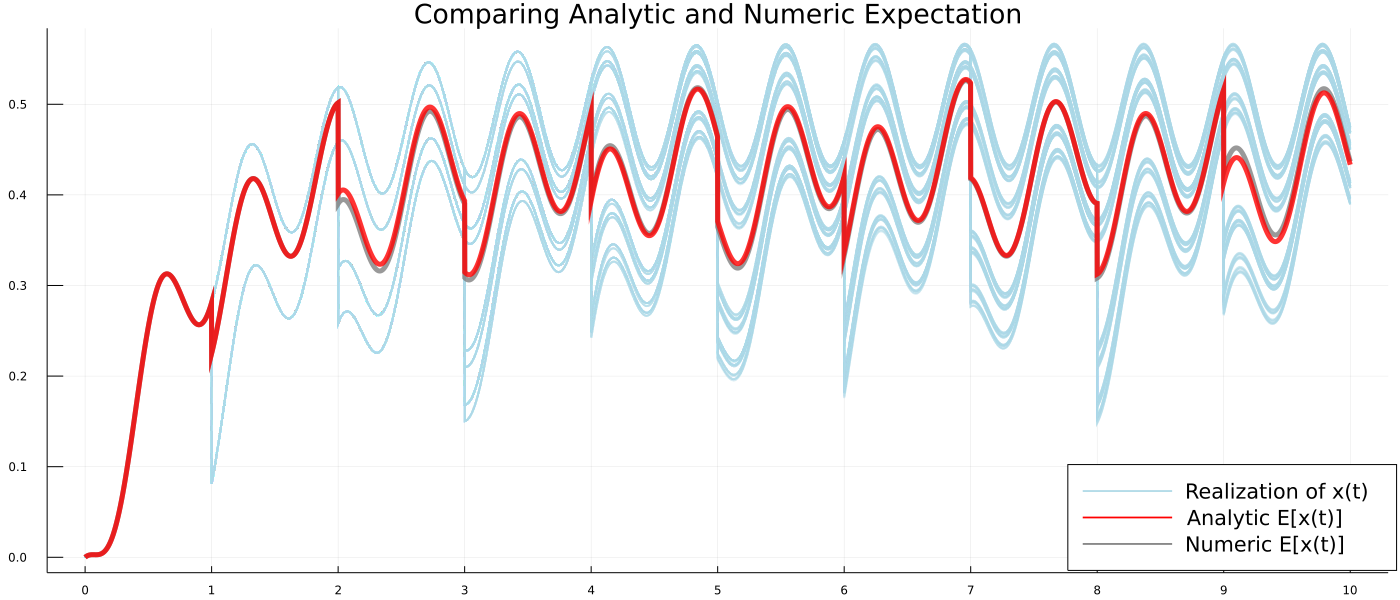
\includegraphics[width=\textwidth]{analytic_expected_p_sin.png}
\end{figure}
In this section we test the formula by plotting it and comparing it to the mean of many simulations.

To avoid overflow in computing $\mathbb{E}[\mathbf{x}(t)]$, we rewrite the formula from Theorem \ref{thm:expectation}.
\begin{flalign*}
 \mathbb{E}[\mathbf{x}(t)] &= I_n(t) 
+ \sum_{k=1}^{n-1} (c\alpha +1)^{n-k}\Big(\frac{c\beta}{c\alpha +1} + I_{k}(t_{k})\Big)e^{-a(t-t_{k})} 
+ (c\alpha + 1)^{n-1} x_0 e^{-a(t-t_0)} 
\end{flalign*}



\bibliographystyle{unsrt}
\bibliography{drinking_references}
\end{document}
